\documentclass[final, letterpaper, 12pt]{article}
%%%%%%%%%%%%%%%%% Idioma y fuentes %%%%%%%%%
\usepackage[spanish,es-tabla]{babel}
\usepackage{fontspec} % para usar fuentes del sistema
\setmainfont{Times New Roman}[
  BoldFont={Times New Roman Bold}, 
  ItalicFont={Times New Roman Italic}, 
  BoldItalicFont={Times New Roman Bold Italic}]
\usepackage{amsmath, amsbsy}
\usepackage{unicode-math}
\setmathfont{Cambria Math}
\usepackage{microtype}
%%%%%%%%%%%%%%%%% Paquetes útiles %%%%%%%%%%
\usepackage{enumitem}
\usepackage[hypcap]{caption}
\captionsetup{font={small,it}, labelfont={small,it},}
\usepackage{graphicx}
\usepackage{multirow}
\usepackage{mathrsfs}
\let\eth\relax %arreglar error linea 20 de esta pagina

\usepackage{listings}
\usepackage{color}
\usepackage{longtable}
\usepackage{fancyhdr}
\usepackage{import}
\usepackage{float}
\usepackage{wrapfig}
\usepackage[margin=0.5in, foot=30pt, head=10pt, bottom=1.3in]{geometry}
\usepackage{hyphenat}
\usepackage[document]{ragged2e}
\usepackage{array}
\usepackage{epstopdf}
\usepackage{imakeidx}
\usepackage[bookmarks=true, hidelinks]{hyperref}
\usepackage{bookmark}
\usepackage{titlesec}
\usepackage{siunitx}
%\usepackage{gensymb}
\usepackage{setspace}
\usepackage{comment}
\usepackage{amsfonts}
\usepackage{makecell}
%\usepackage{subfigure}
\usepackage{subcaption}
\usepackage{placeins}
%%%%%%%%%%%%%%%%% Configuración listings %%%%%%%%%%%%%%%
%%%%%%%%%%%%%%%%% Configuración listings %%%%%%%%%%%%%%%
\definecolor{dkgreen}{rgb}{0,0.6,0}
\definecolor{darkblue}{rgb}{0,0,0.6}
\definecolor{darkgray}{rgb}{0.3,0.3,0.3}
\definecolor{lightgray}{rgb}{0.98,0.98,0.98}
\definecolor{mauve}{rgb}{0.58,0,0.82}
\lstset{
    language=Python,
    basicstyle=\ttfamily\footnotesize,
    keywordstyle=\color{blue},
    commentstyle=\color{dkgreen}\itshape,
    stringstyle=\color{mauve},
    numbers=left,
    numberstyle=\tiny\color{gray},
    breaklines=true,
    breakatwhitespace=true,
    frame=single,
    showstringspaces=false,
    columns=fullflexible,
    tabsize=3,
    literate={á}{{\'a}}1 {é}{{\'e}}1 {í}{{\'i}}1 {ó}{{\'o}}1 {ú}{{\'u}}1 {ñ}{{\~n}}1
}
%%%%%%%%%%%%%%%%% Encabezado y pie %%%%%%%%%%%%%%%
\geometry{left=2cm, right=2cm, top=2.5cm, bottom=3cm}
\pagestyle{fancy}
\fancyhead{}
\fancyfoot{}
\fancyfoot[R]{\thepage}
\fancyhead[R]{ELI348 - Sistemas Electricos de Potencia 3}
\fancyhead[L]{DIE, UTFSM}
\renewcommand{\footrulewidth}{0.9pt}
\setlength{\headheight}{0.09\linewidth}
%%%%%%%%%%%%%%%%% Documento %%%%%%%%%%%%%%%%%%%%%%
\begin{document}
\justifying

\begin{titlepage}
    \begin{center}
        \vspace*{0.8cm}
        
        
\includegraphics[width=0.8\textwidth]{Logo-DIE-vertical-con-fondo.jpg}\\
        \vspace{0.9cm}
        \textbf{{\fontsize{14}{16}\selectfont \LARGE{Sistemas Electricos de Potencia 3}}}\\
        \vspace{0.65cm}
        \headrule
        \vspace{0.4cm}
        \textbf{{\fontsize{14}{16}\selectfont \LARGE{Tarea 2 - Estabilidad de Sistemas Electricos de Potencia}}}\\
        \vspace{0.4cm}
        \headrule
        \vspace{1.4cm}
Autores:\\
        Enrique Guzmán Ortiz, ROL: 202023018-8\\
        Pedro Valenzuela González, ROL: 202023009-9\\
        Joaquín Vargas, ROL: 202023004-8\\
        \vspace{0.7cm}
        Profesor: Victor Hinojosa\\
        \vspace{1cm}
        Valparaíso, Chile\\
        \today  
\end{center}       
\end{titlepage}



\newpage
\tableofcontents 
\newpage
\setlength{\parindent}{0pt} % sin sangría

\section{Objetivos}
\subsection{Objetivo general}

Determinar la capacidad total mínima de compensación dinámica (STATCOM), distribuida en cuatro barras, que elimina las violaciones de trayectoria de tensión (TVI) en las tres contingencias que las producen.

\subsection{Objetivos específicos}

\begin{enumerate}
    \item Implementar una función que, dada una línea fallada, entregue las barras con TVI distinta de cero y su valor, utilizando la envolvente de tensión con $\beta = 0.05$ y $v_{st} = 0.9$ p.u.
    \item Aplicar la función a todas las líneas del sistema (excluyendo los circuitos paralelos), ordenar las contingencias según su TVI total e identificar las barras con mayor TVI acumulada.
    \item Modelar un STATCOM en cada una de las cuatro barras con mayor TVI acumulada, a partir de la plantilla de la librería \textit{Templates} de PowerFactory, y verificar su funcionamiento ante la contingencia Line 28 - 29.
    \item Incorporar la función de cálculo de TVI en una función objetivo con penalización y determinar, mediante MVMO, las cuatro capacidades que eliminan la TVI en las tres contingencias con la menor capacidad total posible.
    \item Implementar la evaluación secuencial con corte anticipado y comparar el número de simulaciones ejecutadas con el caso sin corte anticipado ($3 \times$ número de evaluaciones).
\end{enumerate}
\newpage
\section{Teoría}

\subsection{Estabilidad de tensión de corto plazo y FIDVR}

La estabilidad de tensión es la capacidad de un sistema eléctrico de potencia (SEP) de mantener tensiones aceptables en todas sus barras tras una perturbación. La estabilidad de tensión de corto plazo (STVS, \textit{short-term voltage stability}) abarca una ventana de algunos segundos y está dominada por la dinámica de componentes de respuesta rápida, como motores de inducción, cargas controladas electrónicamente y convertidores HVDC.

En sistemas con alta participación de motores de inducción aparece el fenómeno de recuperación retardada de tensión inducida por fallas (FIDVR, \textit{fault-induced delayed voltage recovery}). Su mecanismo es el siguiente:

\begin{enumerate}
    \item Un cortocircuito deprime la tensión en las barras cercanas a la falla.
    \item Los motores de inducción, al ver reducido su torque eléctrico, se desaceleran.
    \item Tras el despeje de la falla, la tensión comienza a recuperarse y los motores intentan reacelerar, absorbiendo una gran cantidad de potencia reactiva.
    \item Si el sistema no dispone de suficiente soporte de reactivos, la tensión permanece deprimida durante varios segundos, e incluso puede ocurrir estancamiento (\textit{stalling}) de los motores.
\end{enumerate}

El movimiento del rotor de un motor se describe mediante la ecuación de oscilación
\begin{equation}
    \frac{d\omega_r}{dt} = \frac{1}{2H}\left(T_e - T_m\right),
\end{equation}
donde $H$ es la inercia, $T_e$ el torque eléctrico, $T_m$ el torque mecánico y $\omega_r$ la velocidad angular del rotor. Al caer la tensión, $T_e$ (que depende aproximadamente del cuadrado de la tensión) disminuye, $\omega_r$ cae y el deslizamiento aumenta, lo que eleva el consumo de reactivos durante la recuperación.

\subsection{Simulación dinámica RMS}

Los estudios de estabilidad de corto plazo se realizan mediante simulaciones RMS (valores eficaces, secuencia positiva), que son adecuadas para fenómenos entre aproximadamente $0.1$ y $3$ Hz y tienen un costo computacional menor que las simulaciones EMT. El comportamiento del sistema se representa mediante un conjunto de ecuaciones diferenciales-algebraicas (DAE):
\begin{align}
    \dot{\mathbf{x}} &= \mathbf{f}(\mathbf{x}, \mathbf{y}, t), \\
    \mathbf{0} &= \mathbf{g}(\mathbf{x}, \mathbf{y}, t),
\end{align}
donde $\mathbf{x}$ son las variables de estado (máquinas, controles, motores), $\mathbf{y}$ las variables algebraicas (tensiones de barra) y $t$ el tiempo. Las condiciones iniciales $\mathbf{x}(t_0)$ e $\mathbf{y}(t_0)$ se obtienen a partir de un flujo de potencia. Luego, las DAE se resuelven mediante integración numérica con un paso de tiempo $\Delta t$.

El paso de integración influye directamente en la exactitud. Al incorporar equipos basados en electrónica de potencia, como los STATCOM, las constantes de tiempo del control son pequeñas y un paso grande produce resultados oscilatorios o divergentes. Por ello, el paso debe reducirse hasta que una reducción adicional no modifique las curvas.

\subsection{Criterio de recuperación de tensión}

Para juzgar si una recuperación es aceptable se compara la trayectoria de tensión $v(t)$ de cada barra con un criterio o envolvente. Las empresas y operadores definen límites de tensión mínimos que son más permisivos durante los primeros segundos posteriores al despeje y más exigentes a medida que transcurre el tiempo. La inspección visual de cada trayectoria no es práctica en estudios con muchas contingencias, por lo que se emplean índices que cuantifican la violación del criterio.

\subsection{Integral de violación de trayectoria (TVI)}

La TVI (\textit{Trajectory Violation Integral}), propuesta en [1], cuantifica la magnitud y la duración de la violación de la envolvente de tensión. Para la barra $i$ se define de forma general como
\begin{equation}
    \mathrm{TVI}_i = \int_{t_{cl}}^{t_f} \max\!\big(0,\; v_{env}(t) - v_i(t)\big)\, dt,
    \label{eq:tvi}
\end{equation}
donde $t_{cl}$ es el instante de despeje de la falla, $t_f$ el tiempo final de simulación, $v_i(t)$ la tensión de la barra $i$ y $v_{env}(t)$ la envolvente inferior. Las propiedades relevantes son:

\begin{itemize}
    \item $\mathrm{TVI}_i = 0$ si la tensión nunca cae bajo la envolvente.
    \item $\mathrm{TVI}_i > 0$ crece tanto con la profundidad como con la duración de la violación.
    \item Es un indicador local (por barra) que puede agregarse sobre todas las barras.
\end{itemize}

% COMPLETAR: reemplazar por las ecuaciones de la envolvente del paper [1]
% (forma de v_env(t) en función de beta y v_st, e incluir la envolvente
% superior si el paper la define).
En esta tarea la envolvente se construye según [1] con $\beta = 0.05$ y $v_{st} = 0.9$ p.u.

Como las tensiones se obtienen de una simulación, se discretizan en instantes $t_k$ y la integral~\eqref{eq:tvi} se aproxima mediante la regla del trapecio:
\begin{equation}
    \mathrm{TVI}_i \approx \sum_{k} \frac{\Delta_k^{(i)} + \Delta_{k+1}^{(i)}}{2}\,(t_{k+1}-t_k),
    \qquad
    \Delta_k^{(i)} = \max\!\big(0,\; v_{env}(t_k) - v_i(t_k)\big).
\end{equation}
Por esta razón, los valores numéricos dependen levemente del paso de integración, aunque el conjunto de contingencias con TVI y su orden no deberían cambiar. Para evitar que el ruido numérico genere falsos positivos se utiliza una tolerancia pequeña $\varepsilon$ y se considera que existe violación solo si $\mathrm{TVI}_i > \varepsilon$.

La TVI total de una contingencia $k$ es la suma sobre todas las barras:
\begin{equation}
    \mathrm{TVI}_{total}^{(k)} = \sum_{i} \mathrm{TVI}_i^{(k)}.
\end{equation}

\subsection{Análisis de contingencias}

El análisis de contingencias evalúa la respuesta del sistema ante la pérdida de un elemento. En esta tarea cada contingencia consiste en:

\begin{enumerate}
    \item un cortocircuito trifásico franco al $50$\% de la línea en $t = 0$~s;
    \item la desconexión de la línea fallada en $t = 0.1$~s, es decir, un despeje a los $100$~ms.
\end{enumerate}

La apertura de la línea debe modelarse mediante un evento de simulación y no cambiando su estado de servicio en el caso de estudio. De lo contrario, la línea quedaría fuera de servicio de forma permanente y las contingencias siguientes se simularían con una línea menos. Además, los eventos de la corrida anterior deben eliminarse al inicio de cada simulación, para evitar su acumulación.

En los corredores de doble circuito, la contingencia se simula una sola vez sobre el circuito principal y los circuitos paralelos (sufijo \texttt{\_rep}) se excluyen. Las contingencias se ordenan de mayor a menor TVI total, y las barras se ordenan según su TVI acumulada, es decir, la suma de sus aportes en todas las contingencias:
\begin{equation}
    \mathrm{TVI}_i^{acum} = \sum_{k} \mathrm{TVI}_i^{(k)}.
\end{equation}
Las barras con mayor TVI acumulada son las candidatas a alojar compensación dinámica.

\subsection{Compensación dinámica de reactivos: STATCOM}

Un STATCOM (\textit{static synchronous compensator}) es un compensador basado en un convertidor de fuente de tensión (VSC) conectado en derivación a la red. Puede inyectar o absorber potencia reactiva de forma continua y muy rápida, y actúa como fuente de corriente reactiva controlada. Su potencia reactiva puede expresarse como
\begin{equation}
    Q = V \cdot I_q,
\end{equation}
donde $V$ es la tensión en el punto de conexión e $I_q$ la corriente reactiva inyectada. A diferencia de un compensador estático de reactivos (SVC), cuya capacidad es proporcional a $V^2$, el STATCOM mantiene su capacidad de inyección de corriente incluso con tensiones bajas, hasta su límite de corriente. Esto lo hace especialmente adecuado para el soporte durante y después de una falla. En una recuperación retardada de tensión, el STATCOM suministra la potencia reactiva que demandan los motores al reacelerar, lo que acorta el tiempo de recuperación y reduce la TVI.

En PowerFactory, el STATCOM se modela a partir de una plantilla de la librería \textit{Templates}, compuesta por un generador estático (\texttt{ElmGenStat}), un transformador de unidad y un modelo compuesto con el control (DSL). Las condiciones de modelación de esta tarea son:

\begin{itemize}
    \item transformador de unidad de $345/34.5$~kV y $200$~MVA;
    \item eliminación de los capacitores switcheables de la plantilla;
    \item desactivación de la opción \textit{A-stable integration algorithm} en la pestaña RMS, tanto del \texttt{ElmGenStat} como del DSL del control;
    \item reducción del paso de integración de la simulación RMS.
\end{itemize}

La capacidad nominal de cada STATCOM (parámetro \texttt{sgn} del \texttt{ElmGenStat}) es la variable de decisión de la optimización. Un \texttt{ElmGenStat} con potencia nominal nula no es un equipo válido, por lo que si la capacidad es menor que $1$~Mvar el equipo se pone fuera de servicio.

\subsection{Optimización de caja negra}

La TVI se obtiene de una simulación dinámica, por lo que no existe una expresión analítica que relacione las capacidades de los STATCOM con la TVI. Se trata de una función de caja negra: recibe un vector de capacidades y entrega un valor, sin información de gradientes. Para este tipo de problemas se utilizan métodos heurísticos, que solo requieren evaluar la función.

\subsubsection{Formulación del problema}

Se minimiza la capacidad total instalada, sujeto a que la TVI total sea cero en cada contingencia:
\begin{align}
    \min_{Q_1,\dots,Q_4} \quad & \sum_{i=1}^{4} Q_i \\
    \text{s.a.} \quad & \mathrm{TVI}_{total}^{(k)}(Q_1,\dots,Q_4) = 0, \quad k = 1,2,3, \\
    & Q_{min} \le Q_i \le Q_{max},
\end{align}
con $Q_{min} = 0$ y $Q_{max} = 200$~Mvar (potencia nominal del transformador).

\subsubsection{Manejo de restricciones mediante penalización}

Como MVMO no maneja restricciones de forma explícita, la restricción se incorpora a la función objetivo mediante una penalización:
\begin{equation}
    f(\mathbf{Q}) =
    \begin{cases}
        \displaystyle\sum_{i=1}^{4} Q_i & \text{si ninguna contingencia presenta TVI}, \\[2mm]
        10^{6} & \text{si alguna presenta TVI o una simulación no converge}.
    \end{cases}
\end{equation}
Toda solución infactible recibe un valor elevado y es descartada por el algoritmo. Entre las soluciones factibles, se selecciona la de menor capacidad total. Si al finalizar el mejor valor de $f$ es $10^6$, el algoritmo no encontró una solución factible.

\subsubsection{Evaluación secuencial con corte anticipado}

Cada evaluación de $f$ requiere hasta tres simulaciones RMS de $20$~s, una por contingencia, por lo que el tiempo total de optimización depende del número de simulaciones ejecutadas. Para reducirlo se emplea la evaluación secuencial con corte anticipado (Intervención II de [1]): las contingencias se simulan en orden y, en cuanto una presenta TVI, la función retorna la penalización y termina, sin simular las restantes. Una solución que ya viola en una contingencia es infactible, y simular las demás no modifica el valor de $f$.

Las contingencias se evalúan en orden decreciente de severidad (Line 28 - 29, Line 25 - 26, Line 26 - 27), porque la más severa es la que con mayor probabilidad descarta una solución. Si $N_{ev}$ es el número de evaluaciones, sin corte anticipado se ejecutarían $3N_{ev}$ simulaciones. Con corte anticipado el número real $N_{sim}$ cumple
\begin{equation}
    N_{ev} \le N_{sim} \le 3N_{ev},
\end{equation}
y la diferencia $3N_{ev} - N_{sim}$ cuantifica el ahorro.

\subsection{Algoritmo MVMO}

El algoritmo \textit{Mean-Variance Mapping Optimization} (MVMO) es un método heurístico de optimización global que trabaja con una sola solución padre y se caracteriza por usar pocas evaluaciones de la función objetivo, lo que lo hace adecuado cuando cada evaluación es costosa. Sus elementos principales son:

\begin{enumerate}
    \item \textbf{Normalización.} Todas las variables se manejan en el intervalo $[0,1]$. Dentro de la función objetivo se convierten a unidades físicas mediante
    \begin{equation}
        Q_i = Q_{min} + x_i\,(Q_{max} - Q_{min}),
    \end{equation}
    donde $x_i \in [0,1]$ es la variable normalizada.

    \item \textbf{Archivo de soluciones.} El algoritmo almacena las $n$ mejores soluciones encontradas, ordenadas por su valor de $f$. La mejor solución del archivo actúa como padre.

    \item \textbf{Media y varianza.} A partir del archivo se calculan, para cada variable $i$, la media $\bar{x}_i$ y la varianza $v_i$:
    \begin{equation}
        \bar{x}_i = \frac{1}{n}\sum_{j=1}^{n} x_{i,j}, \qquad
        v_i = \frac{1}{n}\sum_{j=1}^{n} \left(x_{i,j} - \bar{x}_i\right)^2 .
    \end{equation}

    \item \textbf{Función de mapeo.} Para generar una nueva solución, a un subconjunto de variables del padre se les asigna un valor aleatorio $x_i \in [0,1]$, que luego se transforma mediante una función de mapeo cuya forma depende de $\bar{x}_i$ y $v_i$:
    \begin{equation}
        h(\bar{x}_i, s_{i1}, s_{i2}, u) = \bar{x}_i\left(1 - e^{-u\,s_{i1}}\right) + \left(1-\bar{x}_i\right) e^{-(1-u)\,s_{i2}},
    \end{equation}
    \begin{equation}
        x_i^{*} = h_x + (1 - h_1 + h_0)\,x_i - h_0,
    \end{equation}
    con $h_x = h(\bar{x}_i, s_{i1}, s_{i2}, x_i)$, $h_0 = h(\bar{x}_i, s_{i1}, s_{i2}, 0)$ y $h_1 = h(\bar{x}_i, s_{i1}, s_{i2}, 1)$. Los factores de forma $s_{i1}$ y $s_{i2}$ se calculan a partir de la varianza, de modo que $s_i \propto -\ln v_i$. Cuando la varianza disminuye (el archivo converge), la función de mapeo concentra los valores generados alrededor de la media; cuando es grande, mantiene la exploración.

    \item \textbf{Actualización.} Si la nueva solución mejora a la peor del archivo, la reemplaza, y el archivo se reordena. El proceso se repite hasta alcanzar el número de evaluaciones definido.
\end{enumerate}

De este modo MVMO equilibra exploración y explotación sin requerir gradientes. Como el algoritmo es estocástico, los resultados dependen de la semilla del generador de números aleatorios. Por ello se fija la semilla $42$ una sola vez, antes de ejecutar MVMO. Si se fijara dentro de la función objetivo, el algoritmo generaría siempre la misma secuencia de números. Distintas ejecuciones o distintos grupos pueden converger a distribuciones de capacidad diferentes con totales similares, y lo relevante es que la solución elimine la TVI y esté bien justificada.

\subsection{Verificación de resultados}

Una solución se considera válida si cumple simultáneamente:

\begin{itemize}
    \item el mejor valor de $f$ es menor que $10^6$;
    \item al simular nuevamente las tres contingencias con las capacidades óptimas, la función de cálculo de la TVI retorna una lista vacía en cada una, es decir, $\mathrm{TVI}_{total}^{(k)} = 0$ para $k = 1, 2, 3$.
\end{itemize}

\newpage
\section{Método y desarrollo}
\subsection{Pregunta a): Función de cálculo de la TVI}

Implementar una función que, dada la línea fallada, entregue las barras con TVI distinta de cero y su valor.

\subsubsection{Metodología}

La función \texttt{calcular\_TVI} se implementó en Python sobre la interfaz de programación de PowerFactory. Recibe como entradas el objeto \texttt{app} y un \textit{string} con el nombre de la línea fallada. Su salida es una lista de listas con una entrada por cada barra cuya TVI es distinta de cero:

\begin{center}
\fbox{\texttt{[[nombre\_barra, TVI], [nombre\_barra, TVI], ...]}}
\end{center}

Si ninguna barra viola la envolvente, la función retorna una lista vacía, y si la simulación no converge retorna \texttt{False}. Este resultado es el criterio que se utilizará en la Pregunta d) para verificar que la compensación es suficiente.

Para cada contingencia, la función ejecuta la siguiente secuencia:

\begin{enumerate}
    \item \textbf{Preparación de los eventos de simulación.} Se reutilizan el evento de cortocircuito (\texttt{ShcLineEvent}) y el de interruptor (\texttt{TripLineEvent}) del caso de estudio, apuntando a la línea fallada, y cualquier otro evento queda fuera de servicio, de modo que no se acumulen fallas de corridas anteriores.
    \item Cortocircuito trifásico franco (resistencia y reactancia nulas) al $50$\,\% de la línea en $t = 0$ s.
    \item Desconexión de la línea en $t = 0{,}1$ s (despeje a los 100 ms), mediante un evento de simulación y no modificando el estado de la línea en el caso de estudio, de modo que las contingencias siguientes no se simulen con una línea menos.
    \item Cálculo de las condiciones iniciales y ejecución de la simulación RMS hasta $t = 20$ s.
    \item Extracción de la magnitud de tensión en p.u. de las 39 barras desde el archivo de resultados.
    \item Construcción de las envolventes según \cite{wildenhues}, con $\beta = 0{,}05$ y $v_{st} = 0{,}9$ p.u. (ecuaciones~\eqref{eq:tlow} y~\eqref{eq:tupp}), cálculo de la TVI de cada barra mediante las ecuaciones~\eqref{eq:tvi} y~\eqref{eq:vv}, y conservación de los valores distintos de cero.
\end{enumerate}

La integral de la ecuación~\eqref{eq:tvi} se evalúa de forma numérica mediante la regla del trapecio sobre las muestras de tensión del archivo de resultados:
\begin{equation}
    \mathrm{TVI}_i \approx \sum_{k} \frac{v_{v,k}^{(i)} + v_{v,k+1}^{(i)}}{2}\,\left(t_{k+1} - t_k\right),
\end{equation}
donde $v_{v,k}^{(i)}$ es la violación instantánea de la barra $i$ en el instante $t_k$. Como el paso de las muestras no es uniforme, se integra directamente sobre el vector de tiempos del archivo de resultados. Una barra se considera con violación solo si su TVI supera una tolerancia de $10^{-6}$ p.u.$\cdot$s, para evitar falsos positivos por ruido numérico.

\paragraph{Ventana de integración.}
La integral se evalúa desde el despeje de la falla ($t = 0{,}1$ s) hasta $t_{end} = 20$ s. Durante el cortocircuito, las barras cercanas a la falla presentan tensiones inferiores a la envolvente en todas las contingencias, por lo que incluir ese intervalo sumaría una violación que no corresponde a la recuperación posterior. Esta decisión se verificó con la contingencia Line 28 - 29: integrando desde $t = 0$ s el total fue $0{,}204$, aproximadamente el doble del valor referencial de la guía, mientras que integrando desde el despeje fue $0{,}0969$.

El código completo de la función se encuentra en el Anexo~\ref{anexo:codigo_a}.

\subsubsection{Resultados}

La Tabla~\ref{tab:salida_a} muestra la salida de la función para la contingencia Line 28 - 29, y la Tabla~\ref{tab:tvi_total_a} el valor de su TVI total, calculada como la suma de la TVI de todas las barras (ecuación~\eqref{eq:tvitot}).

\begin{table}[H]
    \centering
    \caption{Salida de \texttt{calcular\_TVI} ante la contingencia Line 28 - 29.}
    \label{tab:salida_a}
    \begin{tabular}{|l|c|}
        \hline
        Barra & TVI [p.u.$\cdot$s] \\
        \hline
        Bus 26 & 0.000197 \\
        \hline
        Bus 28 & 0.020780 \\
        \hline
        Bus 29 & 0.040256 \\
        \hline
        Bus 38 & 0.035617 \\
        \hline
    \end{tabular}
\end{table}

\begin{table}[H]
    \centering
    \caption{TVI total de la contingencia Line 28 - 29.}
    \label{tab:tvi_total_a}
    \begin{tabular}{|l|c|}
        \hline
        Contingencia & TVI total [p.u.$\cdot$s] \\
        \hline
        Line 28 - 29 & 0.096850 \\
        \hline
    \end{tabular}
\end{table}

La Figura~\ref{fig:bus29_a} ilustra el cálculo para la barra 29, la de mayor TVI en esta contingencia. Durante el cortocircuito (0 a 0.1 s) la tensión cae desde 1.05 p.u. a valores cercanos a 0.2 p.u., muy por debajo de la envolvente, por lo que ese intervalo no se considera. Tras el despeje, las áreas sombreadas entre la trayectoria y los límites de la envolvente corresponden a la TVI de la barra.

\begin{figure}[H]
    \centering
    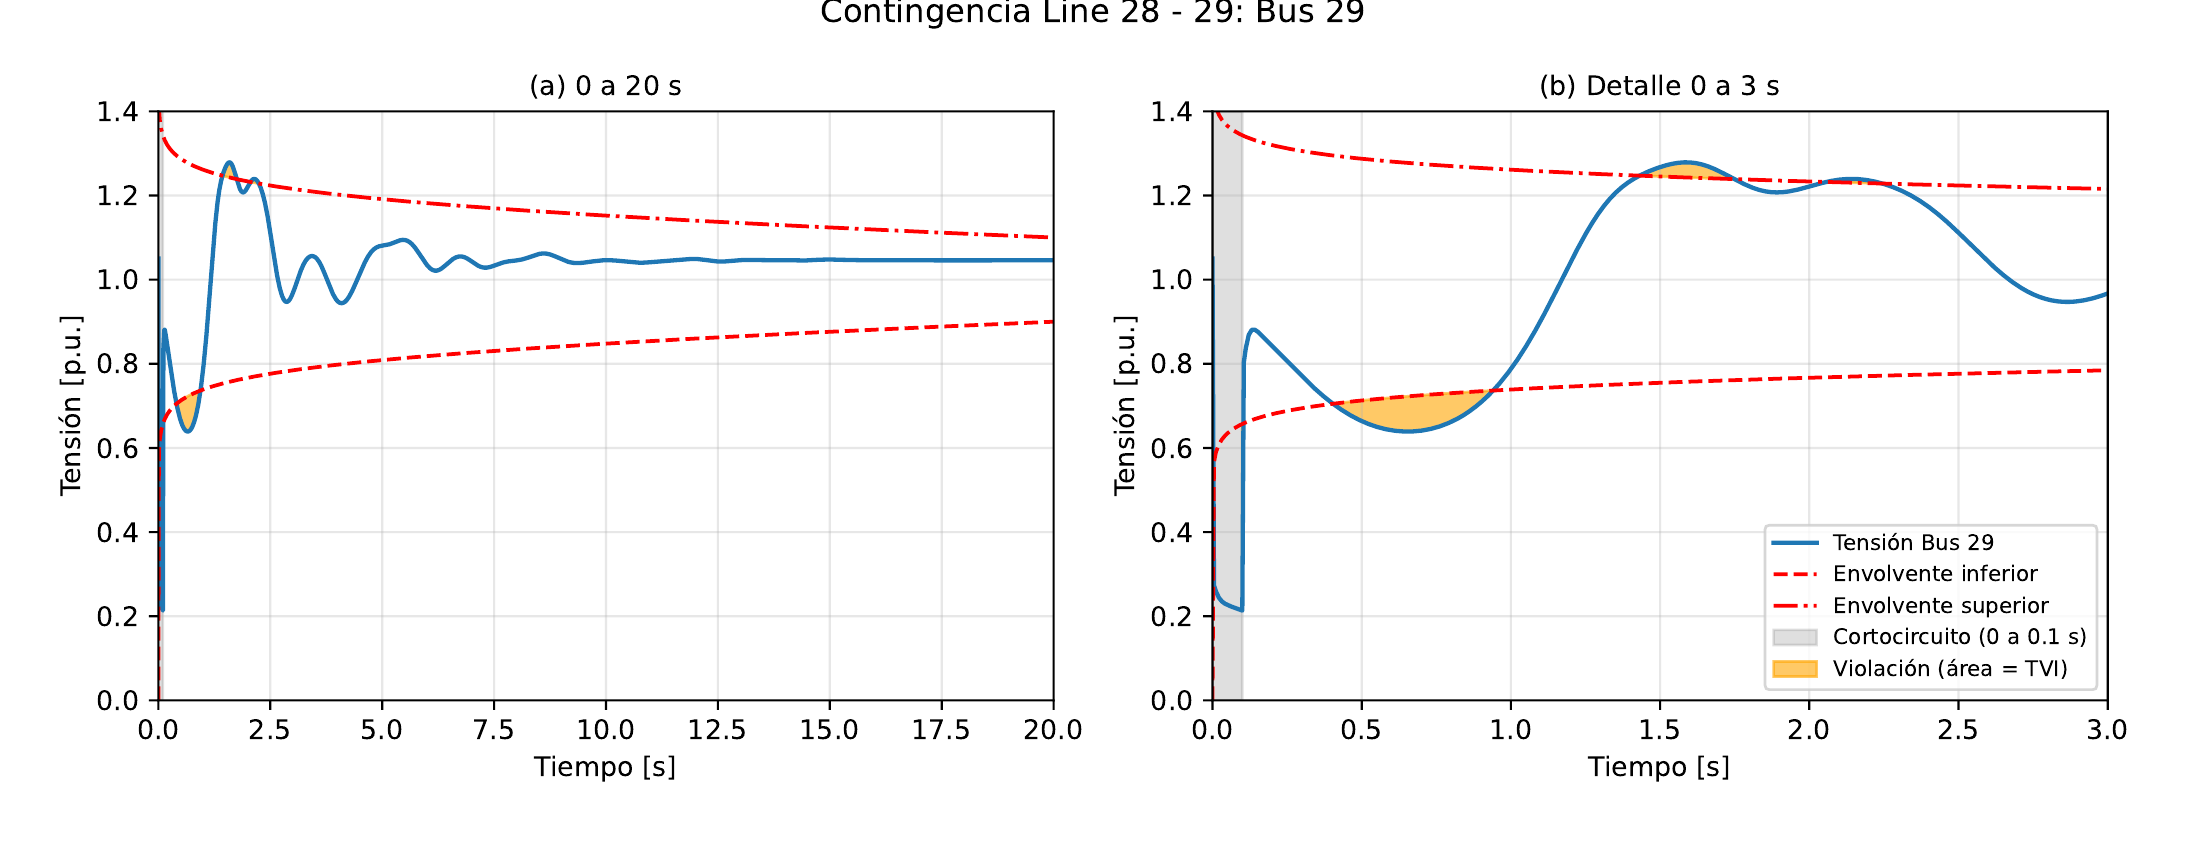
\includegraphics[width=\textwidth]{Desarrollo/Imagenes Informe/tvi_bus29_line_28_29.png}
    \caption{Trayectoria de tensión de la barra 29 y envolvente ante la contingencia Line 28 - 29: (a) vista completa y (b) detalle de los primeros 3 s. El área sombreada corresponde a la TVI de la barra.}
    \label{fig:bus29_a}
\end{figure}

Para una línea cuya contingencia no produce violaciones de la envolvente, la función retorna una lista vacía, \texttt{[]}.

\subsubsection{Comentarios}

El valor de TVI total obtenido para la contingencia Line 28 - 29 es $0{,}0969$, un $6$\,\% inferior al valor referencial de la guía ($0{,}1034$). El orden de magnitud coincide, y las diferencias menores pueden atribuirse al paso de integración de la simulación y al método de integración numérica empleado.

La mayor parte de la TVI se concentra en las barras 28 y 29, que son los terminales de la línea fallada. La barra 26 aporta un valor marginal ($0{,}000197$, cerca del $0{,}2$\,\% del total). Además aparece la barra 38, una barra de generación de 16.5 kV conectada eléctricamente a la barra 29, cuya tensión acompaña la de esta última.

Para que cada contingencia se simule de forma independiente, la función no acumula eventos de corridas previas y abre la línea mediante un evento de simulación. Además, solo conserva las barras con TVI distinta de cero. Esto permite usar directamente el largo de la lista de salida como criterio de factibilidad en la Pregunta d): una lista vacía indica que ninguna barra viola la envolvente.

Una simulación completa de una contingencia tarda aproximadamente 5 s: 0.9 s en el cálculo de condiciones iniciales, 0.6 s en la simulación RMS y 3.4 s en la lectura de resultados. Este valor es relevante para planificar el número de evaluaciones de la optimización de la Pregunta d).
\newpage
\section{Crítica y comentarios}
\input{Desarrollo/Critica y comentarios}
\newpage
\section{Bibliografía}
\addcontentsline{toc}{section}{Referencias}
\begin{thebibliography}{100}
    \bibitem{Cita} S. Wildenhues, J. L. Rueda and I. Erlich, ``Optimal Allocation and Sizing of Dynamic Var Sources Using Heuristic Optimization,'' \textit{IEEE Transactions on Power Systems}, vol. 30, no. 5, pp. 2538--2546, Sept. 2015.
\end{thebibliography}
\newpage
\section{Apéndices}

\subsection{Código de la Pregunta a): función \texttt{calcular\_TVI}}
\label{anexo:codigo_a}

\definecolor{gray}{gray}{0.5}

\begin{lstlisting}
import numpy as np

BETA = 0.05
VST = 0.9
T_FALLA = 0.0
T_DESPEJE = 0.1
T_END = 20.0
TOL = 1e-6

_trapz = getattr(np, "trapezoid", None) or np.trapz


def envolvente(t, beta=BETA, vst=VST, t_end=T_END):
    """Envolventes inferior y superior segun Wildenhues et al."""
    t = np.asarray(t, dtype=float)
    t_low = ((t / t_end) * np.exp(t / t_end)) ** beta / np.exp(beta) * vst
    t_upp = 2.0 - t_low
    return t_low, t_upp


def calcular_TVI(app, nombre_linea):
    """Retorna [[barra, TVI], ...] con TVI != 0, [] si no hay
    violaciones o False si la simulacion no converge."""
    try:
        # 1. Preparar eventos (se reutilizan los del caso de estudio)
        evt = app.GetFromStudyCase("IntEvt")
        linea = app.GetCalcRelevantObjects(nombre_linea + ".ElmLne")[0]
        falla = evt.GetContents("ShcLineEvent*")[0]
        disparo = evt.GetContents("TripLineEvent*")[0]
        for e in evt.GetContents():
            e.outserv = 1
        falla.outserv = 0
        disparo.outserv = 0

        # 2. Cortocircuito trifasico franco al 50 % en t = 0
        falla.p_target = linea
        falla.time = T_FALLA
        falla.i_shc = 0
        falla.R_f = 0.0
        falla.X_f = 0.0
        falla.fshcloc = 50.0

        # 3. Apertura de la linea en t = 0.1 s (evento, no outserv)
        disparo.p_target = linea
        disparo.time = T_DESPEJE
        disparo.i_switch = 0

        # 4. Condiciones iniciales y simulacion RMS hasta 20 s
        inc = app.GetFromStudyCase("ComInc")
        sim = app.GetFromStudyCase("ComSim")
        inc.iopt_sim = "rms"
        if inc.Execute() != 0:
            return False
        sim.tstop = T_END
        if sim.Execute() != 0:
            return False

        # 5. Extraer tensiones en p.u. de las barras
        res = inc.p_resvar
        res.Load()
        n = res.GetNumberOfRows()
        t = np.array([res.GetValue(i, -1)[1] for i in range(n)])
        barras = app.GetCalcRelevantObjects("*.ElmTerm")
        V = {}
        for b in barras:
            col = res.FindColumn(b, "m:u")
            if col < 0:
                continue
            V[b.loc_name] = np.array(
                [res.GetValue(i, col)[1] for i in range(n)])
        res.Release()
    except Exception:
        return False

    # 6. Envolventes y TVI por barra (desde el despeje hasta t_end)
    mask = t >= T_DESPEJE
    tc = t[mask]
    t_low, t_upp = envolvente(tc)

    salida = []
    for nombre, v in V.items():
        vc = v[mask]
        viol = np.maximum(t_low - vc, 0.0) + np.maximum(vc - t_upp, 0.0)
        tvi = float(_trapz(viol, tc))
        if tvi > TOL:
            salida.append([nombre, tvi])
    return salida
\end{lstlisting}

\end{document}